\documentclass[]{article}
\usepackage[T2A]{fontenc}
\usepackage[utf8]{inputenc}
\usepackage[russian]{babel}
\usepackage{amsmath}
\usepackage{amsmath, amsfonts, amssymb, amsthm, mathtools}
\usepackage[left=20mm, top=15mm, right=15mm, bottom=20mm, nohead, nofoot]{geometry}
\usepackage{graphicx}
\usepackage{float}%"Плавающие" картинки
\usepackage{wrapfig}%Обтекание фигур (таблиц, картинок и прочего)
\usepackage{listings}
%opening
\begin{document}
	\begin{titlepage}
		\begin{center}
			\large Санкт-Петербургский политехнический университет Петра Великого \\
			\large Физико-механический институт \\
			\large Высшая школа теоретической механики и математической физики \\[2cm] % [] - отступ
			\large Направление подготовки \\
			\large 01.03.03 Механика и математическое моделирование \\[2cm]
			\LARGE \textbf {Отчёт по лабораторной работе №4} \\[0.5cm]
			\LARGE \textbf {Тема: "Интерполяционные полиномы"} \\[0.5cm]
			\large Дисциплина "Вычислительная механика" \\[4cm]
		\end{center}
		\begin{minipage}{0.25\textwidth} % врезка в половину ширины текста
			\begin{flushright}
				\large\textbf{Выполнил:}\\
				\large Работинский А.Д. \\
				\large {Группа:} 5030103/10001 \\
				\large \textbf{Преподаватель:}\\
				\large Е.Ю. Витохин
			\end{flushright}
		\end{minipage}
		\mbox{}
		\vfill
		\begin{center}
			\large Санкт-Петербург \\
			\large 2022 
		\end{center} 
	\end{titlepage}
	\newpage
	\section*{1) Постановка задачи}
		Требуется отыскать функции формы для всех узлов данного конечного элемента, провести проверку путем непосредственной подстановки узловых точек в полученные функции, построить визуализацию. Рассматриваемый конечный элемент: линейный тетраэдр.\\
		\begin{center}
			Перемещения внутри линейного тетраэдра: $u=A+Bx+Cy+Dz+Exy+Fxz+Gyz+Hxyz$
			\begin{figure}[H]
				\centering
				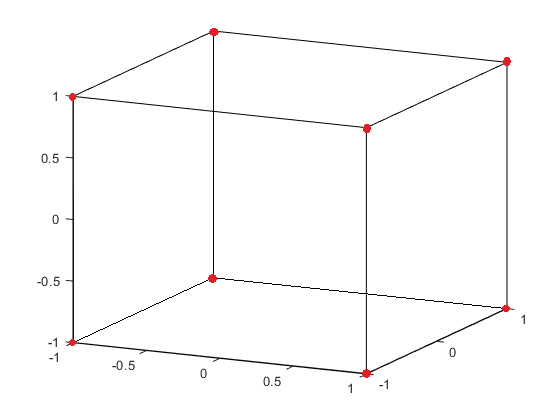
\includegraphics[width=0.3\textwidth]{tetr}
				\caption{Линейный тетраэдр с отмеченными узлами}
				\label{рис. 1}
			\end{figure}
			Узлы тетраэдра:\\
			\begin{tabular}{| p{1cm} | p{1cm}| p{1cm} |p{1cm} |}
				\hline
				Номер узла & X & Y & Z\\
				\hline
				1 & -1 & -1 & -1\\
				\hline
				2 &	-1 & -1	& 1\\
				\hline
				3 & -1 &  1 & -1\\
				\hline
				4 & -1 &  1	& 1\\
				\hline
				5 &	  1 & -1	& -1\\
				\hline
				6 &   1 & -1 & 1\\
				\hline
				7 &	  1 &  1 & -1\\
				\hline
				8 &	  1 &  1	& 1\\
				\hline
			\end{tabular}\\[2\baselineskip]
			Функция формы для $i \text{-ого}$ узла должна удовлетворять следущему равенству:\\
			$N_m(x_m,y_m,z_m)=1$
			\[N_m(x_i,y_i,z_i)=0 \quad (i\neq m)\]
		\end{center}
	\section*{2) Решение}
		Для каждого узла из 8 выше представленных можно записать 8 уравнений исходя из свойств:\\
		\begin{center}
			$N_m(x_i,y_i,z_i)=1 \quad (i=m) \text{(1 уравнение) и } N_m(x_i,y_i,z_i)=1 \quad (i\neq m) \text{(7 уравнений)} $
		\end{center}
		Получим систему следующего вида:\\
		\[\begin{pmatrix}
			1&x_1&y_1&z_1&x_1y_1&x_1z_1&y_1z_1&x_1y_1z_1\\
			1&x_2&y_2&z_2&x_2y_2&x_2z_2&y_2z_2&x_2y_2z_2\\
			1&x_3&y_3&z_3&x_3y_3&x_3z_3&y_3z_3&x_3y_3z_3\\
			1&x_4&y_4&z_4&x_4y_4&x_4z_4&y_4z_4&x_4y_4z_4\\
			1&x_5&y_5&z_5&x_5y_5&x51z_5&y_5z_5&x_5y_5z_5\\
			1&x_6&y_6&z_6&x_6y_6&x_6z_6&y_6z_6&x_6y_6z_6\\
			1&x_7&y_7&z_7&x_7y_7&x_7z_7&y_7z_7&x_7y_7z_7\\
			1&x_8&y_8&z_8&x_8y_8&x_8z_8&y_8z_8&x_8y_8z_8\\
		\end{pmatrix}
		\begin{pmatrix}
			A_1&A_2&A_3&A_4&A_5&A_6&A_7&A_8\\
			B_1&B_2&B_3&B_4&B_5&B_6&B_7&B_8\\
			C_1&C_2&C_3&C_4&C_5&C_6&C_7&C_8\\
			D_1&D_2&D_3&D_4&D_5&D_6&D_7&D_8\\
			E_1&E_2&E_3&E_4&E_5&E_6&E_7&E_8\\
			F_1&F_2&F_3&F_4&F_5&F_6&F_7&F_8\\
			G_1&G_2&G_3&G_4&G_5&G_6&G_7&G_8\\
			H_1&H_2&H_3&H_4&H_5&H_6&H_7&H_8\\
		\end{pmatrix}
		=[E]\]
		\newpage
		Перепишем систему более компактно:\\
		\begin{center}
			$[X][A]=[E] \quad | \quad [X]* \quad \Rightarrow$ \fbox {$[A]=[X]^{-1}$}
		\end{center}
		Получившася матрица коэффициентов:
		\begin{center}
			\begin{figure}[H]
				\centering
				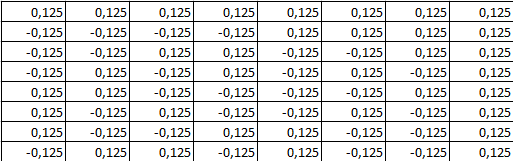
\includegraphics[width=0.6\textwidth]{kofs}
				\caption{Матрица коэффициентов}
				\label{рис. 2}
			\end{figure}
		\end{center}
		Тогда составив вектор-столбец $\approx$ интерполяционному многочлену: $ [P]^T=[1 \quad x \quad y \quad z \quad xy \quad xz \quad yz \quad xyz]$\\
		\begin{center}
			Найдем функции формы следующим обраом:\\
			$[\widetilde{N}]=[P]^T*[A]$\\
			Тогда, полученные функции формы:\\
			\[\fbox{N_1=\frac{1}{8}((x*y) - y - z - x + (x*z) + (y*z) - (x*y*z) + 1)}\]
			\[\fbox{N_2=\frac{1}{8}(z - y - x + (x*y) - (x*z) - (y*z) + (x*y*z) + 1)}\]
			\[\fbox{N_3=\frac{1}{8}(y - x - z - (x*y) + (x*z) - (y*z) + (x*y*z) + 1)}\]
			\[\fbox{N_4=\frac{1}{8}(y - x + z - (x*y) - (x*z) + (y*z) - (x*y*z) + 1)}\]
			\[\fbox{N_5=\frac{1}{8}(x - y - z - (x*y) - (x*z) + (y*z) + (x*y*z) + 1)}\]
			\[\fbox{N_6=\frac{1}{8}(x - y + z - (x*y) + (x*z) - (y*z) - (x*y*z) + 1)}\]
			\[\fbox{N_7=\frac{1}{8}(x + y - z + (x*y) - (x*z) - (y*z) - (x*y*z) + 1)}\]
			\[\fbox{N_8=\frac{1}{8}(x + y + z + (x*y) + (x*z) + (y*z) + (x*y*z) + 1)}\]	
		\end{center}
	\newpage
	\section*{3) Проверка результатов по визулизации}
		Спроецируем значения функций форм на исходный конечный элемент:\\
			\begin{center}
				\begin{figure}[H]
					\centering
					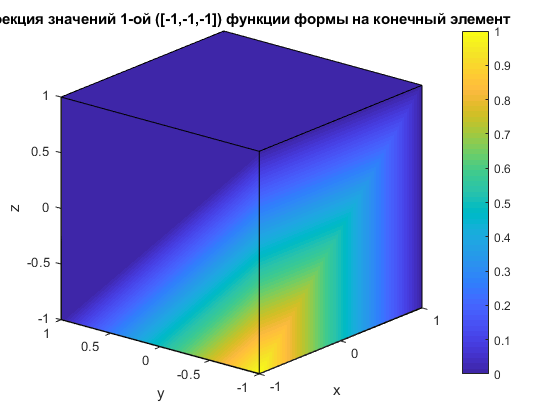
\includegraphics[width=0.6\textwidth]{1}
					\caption{Проекция значений 1ой функции формы на конечный элемент}
					\label{рис. 3}
				\end{figure}
			\end{center}
		
			\begin{center}
				\begin{figure}[H]
					\centering
					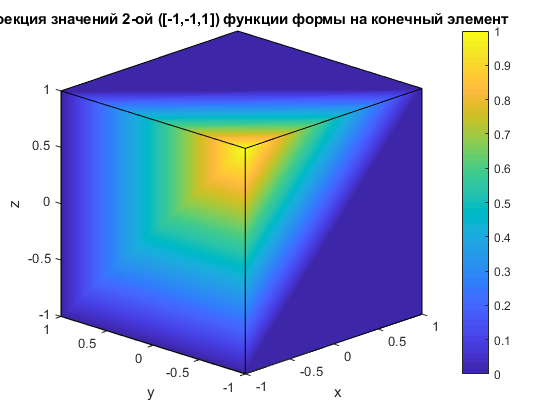
\includegraphics[width=0.6\textwidth]{2}
					\caption{Проекция значений 2ой функции формы на конечный элемент}
					\label{рис. 4}
				\end{figure}
			\end{center}
		
			\begin{center}
				\begin{figure}[H]
					\centering
					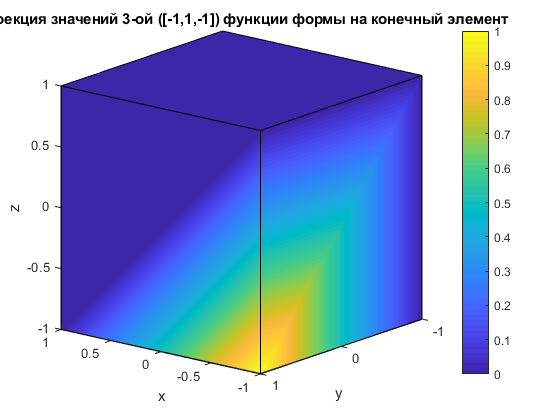
\includegraphics[width=0.6\textwidth]{3}
					\caption{Проекция значений 3ой функции формы на конечный элемент}
					\label{рис. 5}
				\end{figure}
			\end{center}
		
			\begin{center}
				\begin{figure}[H]
					\centering
					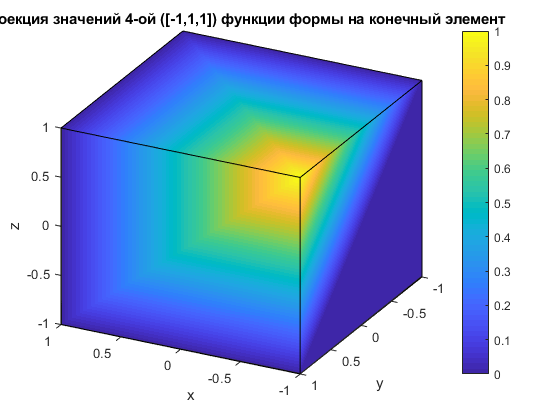
\includegraphics[width=0.6\textwidth]{4}
					\caption{Проекция значений 4ой функции формы на конечный элемент}
					\label{рис. 6}
				\end{figure}
			\end{center}
		
			\begin{center}
				\begin{figure}[H]
					\centering
					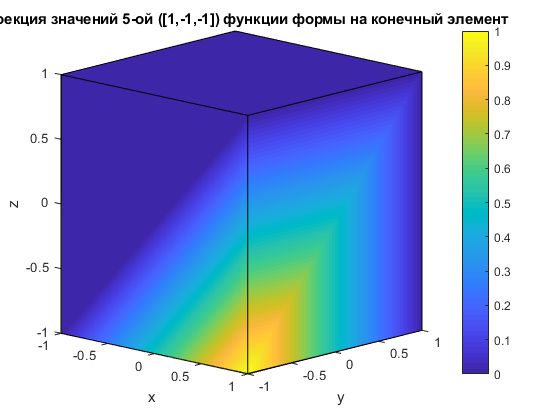
\includegraphics[width=0.6\textwidth]{5}
					\caption{Проекция значений 5ой функции формы на конечный элемент}
					\label{рис. 7}
				\end{figure}
			\end{center}
		
			\begin{center}
				\begin{figure}[H]
					\centering
					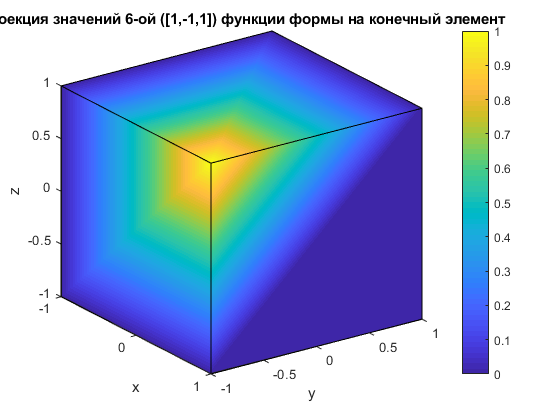
\includegraphics[width=0.6\textwidth]{6}
					\caption{Проекция значений 6ой функции формы на конечный элемент}
					\label{рис. 8}
				\end{figure}
			\end{center}
			
			\begin{center}
				\begin{figure}[H]
					\centering
					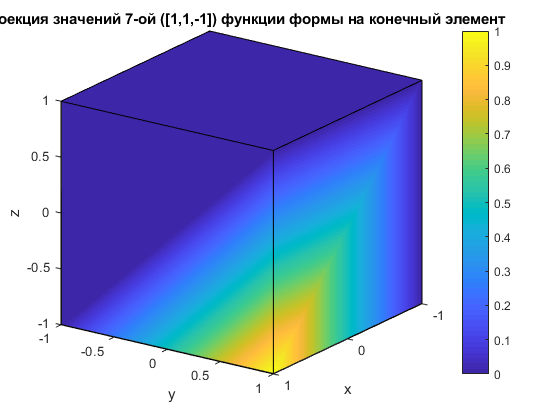
\includegraphics[width=0.6\textwidth]{7}
					\caption{Проекция значений 7ой функции формы на конечный элемент}
					\label{рис. 9}
				\end{figure}
			\end{center}
			
			\begin{center}
				\begin{figure}[H]
					\centering
					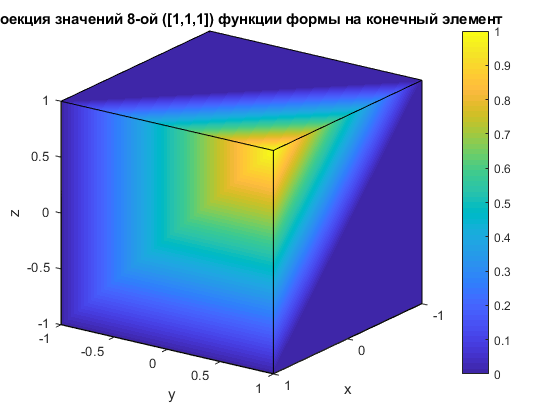
\includegraphics[width=0.6\textwidth]{8}
					\caption{Проекция значений 8ой функции формы на конечный элемент}
					\label{рис. 10}
				\end{figure}
			\end{center}
		\section*{4) Выводы}
		Из 3 пункта видно, что найденные функции форм удовлетворяют свойствам, что говорит о верности проведенных вычислений.
		\newpage
		\section*{5) Код (выполнен в MATLAB)}
		\begin{lstlisting}
X=zeros(8);
x_nde=[];
y_nde=[];
z_nde=[];
			
x_nde(end+1)=-1;
y_nde(end+1)=-1;
z_nde(end+1)=-1;

x_nde(end+1)=-1;
y_nde(end+1)=-1;
z_nde(end+1)=1;

x_nde(end+1)=-1;
y_nde(end+1)=1;
z_nde(end+1)=-1;

x_nde(end+1)=-1;
y_nde(end+1)=1;
z_nde(end+1)=1;

x_nde(end+1)=1;
y_nde(end+1)=-1;
z_nde(end+1)=-1;

x_nde(end+1)=1;
y_nde(end+1)=-1;
z_nde(end+1)=1;

x_nde(end+1)=1;
y_nde(end+1)=1;
z_nde(end+1)=-1;

x_nde(end+1)=1;
y_nde(end+1)=1;
z_nde(end+1)=1;
			
X(:,1)=1;
for i=1:8
X(i,2)=x_nde(i);
X(i,3)=y_nde(i);
X(i,4)=z_nde(i);
X(i,5)=x_nde(i)*y_nde(i);
X(i,6)=x_nde(i)*z_nde(i);
X(i,7)=y_nde(i)*z_nde(i);
X(i,8)=x_nde(i)*y_nde(i)*z_nde(i);
end
A=zeros(8);
A=inv(X);
syms x y z;
P=[1;x;y;z;x*y;x*z;y*z;x*y*z];
P=P.';
N=P*A
			
f(1)={@(x,y,z) (x.*y)/8 - y./8 - z./8 - x./8 + (x.*z)./8 + (y.*z)./8 - (x.*y.*z)./8 + 1/8};
f(2)={@(x,y,z) z./8 - y./8 - x./8 + (x.*y)./8 - (x.*z)./8 - (y.*z)./8 + (x.*y.*z)./8 + 1/8};
f(3)={@(x,y,z) y./8 - x./8 - z./8 - (x.*y)./8 + (x.*z)./8 - (y.*z)./8 + (x.*y.*z)./8 + 1/8};
f(4)={@(x,y,z) y./8 - x./8 + z./8 - (x.*y)./8 - (x.*z)./8 + (y.*z)./8 - (x.*y.*z)./8 + 1/8};
f(5)={@(x,y,z) x./8 - y./8 - z./8 - (x.*y)./8 - (x.*z)./8 + (y.*z)./8 + (x.*y.*z)./8 + 1/8};
f(6)={@(x,y,z) x./8 - y./8 + z./8 - (x.*y)./8 + (x.*z)./8 - (y.*z)./8 - (x.*y.*z)./8 + 1/8};
f(7)={@(x,y,z) x./8 + y./8 - z./8 + (x.*y)./8 - (x.*z)./8 - (y.*z)./8 - (x.*y.*z)./8 + 1/8};
f(8)={@(x,y,z) x./8 + y./8 + z./8 + (x.*y)./8 + (x.*z)./8 + (y.*z)./8 + (x.*y.*z)./8 + 1/8};
for i=1:8
figure()
hold on
fill3([1 1 -1 -1],[1 1 1 1],[-1 1 1 -1],[f{i}(x_nde(7),y_nde(7),z_nde(7))
,f{i}(x_nde(8),y_nde(8),z_nde(8)),f{i}(x_nde(4),y_nde(4),z_nde(4))
,f{i}(x_nde(3),y_nde(3),z_nde(3))]);
fill3([-1 -1 -1 -1],[1 1 -1 -1],[-1 1 1 -1],[f{i}(x_nde(3),y_nde(3),z_nde(3)),
f{i}(x_nde(4),y_nde(4),z_nde(4)),f{i}(x_nde(2),y_nde(2),z_nde(2))
,f{i}(x_nde(1),y_nde(1),z_nde(1))]);
fill3([-1 -1 1 1],[-1 -1 -1 -1],[-1 1 1 -1],[f{i}(x_nde(1),y_nde(1),z_nde(1))
,f{i}(x_nde(2),y_nde(2),z_nde(2)),f{i}(x_nde(6),y_nde(6),z_nde(6))
,f{i}(x_nde(5),y_nde(5),z_nde(5))]);
fill3([1 1 1 1],[-1 -1 1 1],[-1 1 1 -1],[f{i}(x_nde(5),y_nde(5),z_nde(5))
,f{i}(x_nde(6),y_nde(6),z_nde(6)),f{i}(x_nde(8),y_nde(8),z_nde(8))
,f{i}(x_nde(7),y_nde(7),z_nde(7))]);
fill3([-1 -1 1 1],[1 -1 -1 1],[1 1 1 1],[f{i}(x_nde(4),y_nde(4),z_nde(4))
,f{i}(x_nde(2),y_nde(2),z_nde(2)),f{i}(x_nde(6),y_nde(6),z_nde(6))
,f{i}(x_nde(8),y_nde(8),z_nde(8))]);
fill3([-1 -1 1 1],[1 -1 -1 1],[-1 -1 -1 -1],[f{i}(x_nde(3),y_nde(3),z_nde(3))
,f{i}(x_nde(1),y_nde(1),z_nde(1)),f{i}(x_nde(5),y_nde(5),z_nde(5))
,f{i}(x_nde(7),y_nde(7),z_nde(7))]);
colorbar;
xlabel('x');
ylabel('y');
zlabel('z');
view(125,21);
end
		\end{lstlisting}
\end{document}
